\subsection{Prodotto matrice-vettore}
Il prodotto matrice-vettore é un algoritmo dell'algebra lineare che definisce, come desumibile dal nome, il prodotto tra una matrice ed un vettore. Tale prodotto produce un nuovo vettore.
Formalmente, sia $A \in M_{m,n}, x \in \mathbb{K}^n$, allora $A\cdot x = b$, dove $b \in \mathbb{K}^m$.
Il vettore risultante $b$ viene calcolato dal seguente algoritmo:
\begin{lstlisting}
for i from 0 to m do
    for j from 0 to n do
        b[i] = b[i] + A[i][j] * x[j];
\end{lstlisting}
Ecco di seguito una rappresentazione visiva delle posizioni degli indici $i$ e $j$.
\begin{figure}[h]
    \centering
    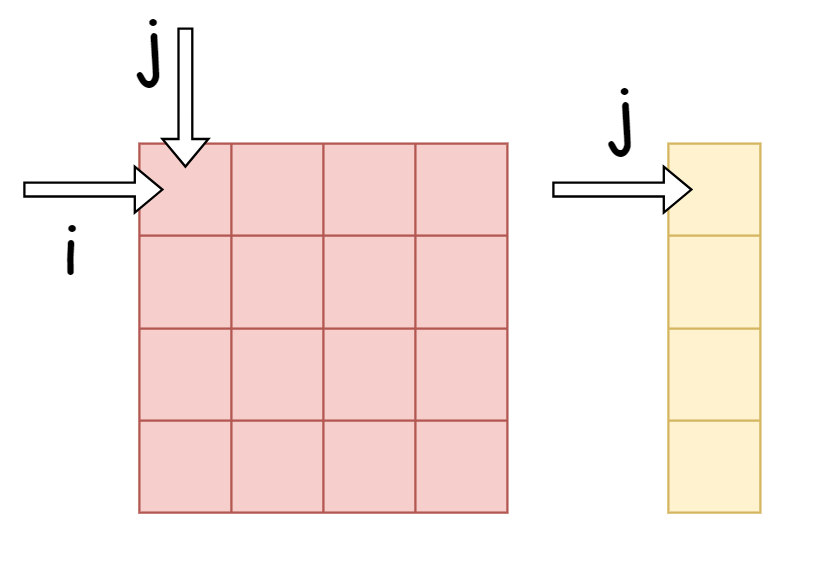
\includegraphics[width=0.4\linewidth]{PrimaItr.png}
    \caption{Primo passo}
    \label{fig:enter-label}    
\end{figure}
\begin{figure}[h]
    \centering
    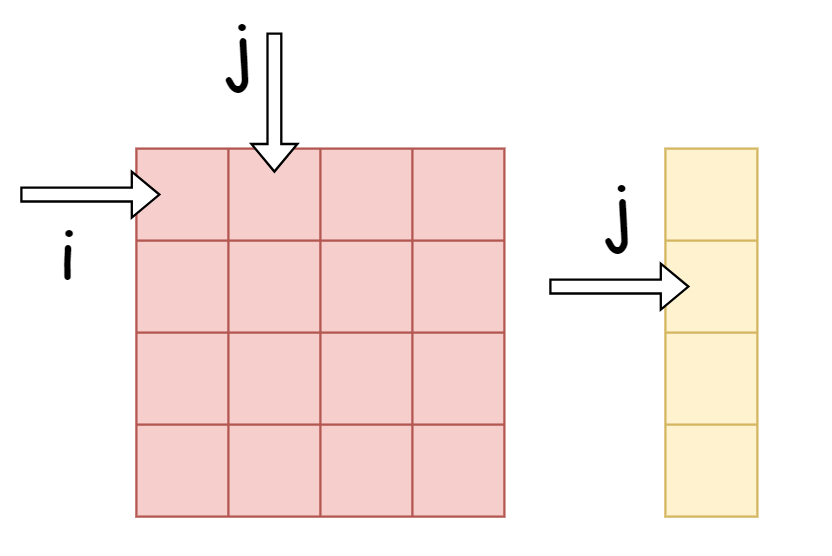
\includegraphics[width=0.4\linewidth]{SecondaItr.png}
    \caption{Secondo passo}
    \label{fig:enter-label}    
\end{figure}
\begin{figure}[h]
    \centering
    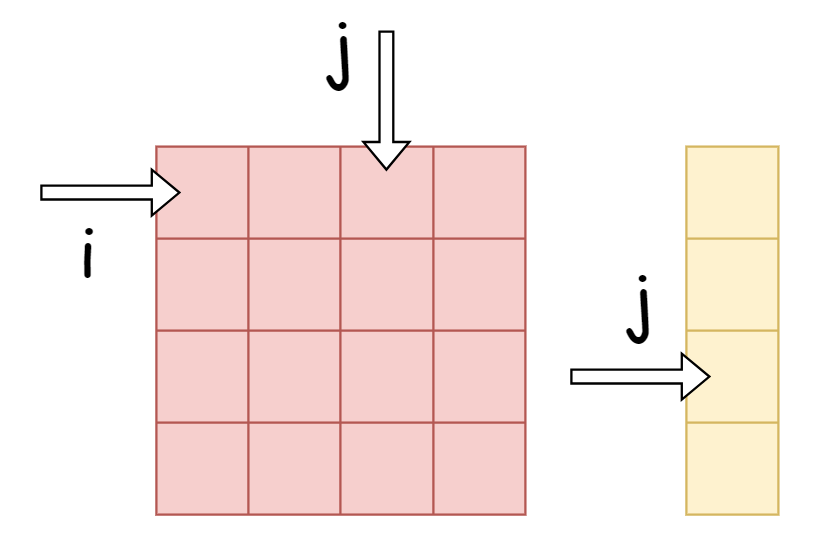
\includegraphics[width=0.4\linewidth]{Terza.png}
    \caption{Terzo passo}
    \label{fig:enter-label}    
\end{figure}
\begin{figure}[h]
    \centering
    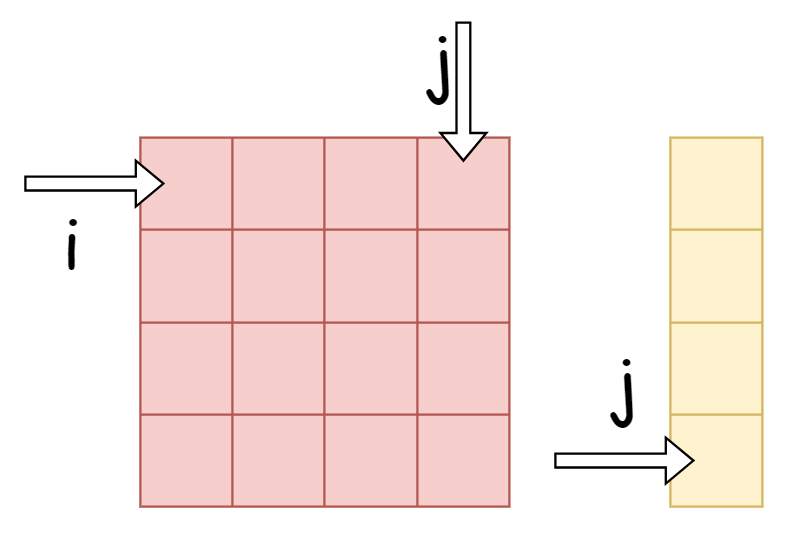
\includegraphics[width=0.4\linewidth]{QuartaItr.png}
    \caption{Quarto passo}
    \label{fig:enter-label}    
\end{figure}
\begin{figure}[h]
    \centering
    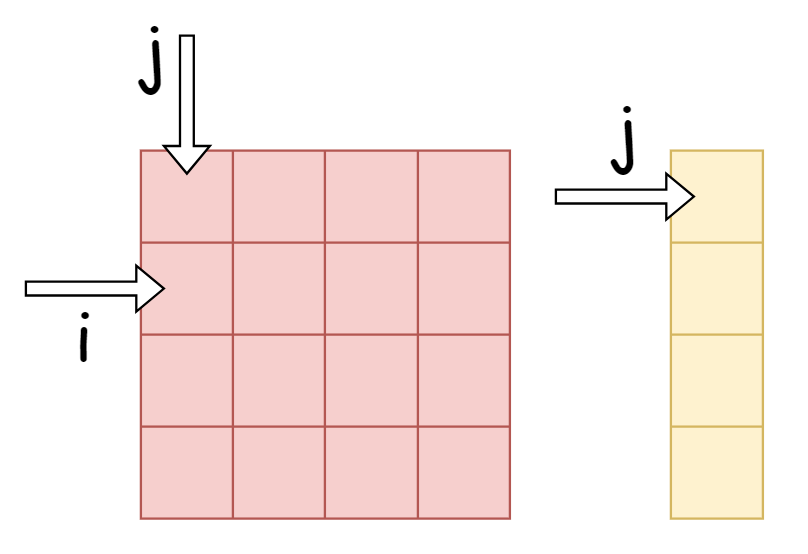
\includegraphics[width=0.4\linewidth]{QuintaItr.png}
    \caption{Quinto passo}
    \label{fig:enter-label}    
\end{figure}


\subsection{Approccio alla risoluzione}
Si può facilmente notare che i passi dell'algoritmo sono perfettamente indipendenti tra loro: ciò significa che è possibile una loro suddivisione tra esecutori.

La suddivisione proposta sfrutta la API OpenMP, la quale permette la parallelizzazione in calcolatori MIMD a memoria condivisa mediante la suddivisione di un processo in thread.
